\section{Potential solutions and trade-offs}
\label{sec:solution}

\ad{this is in super messed up state. I am currently organizing this sections to
different parts such as : anti-phishing(Section 6 now), data confidentiality
etc}

\begin{figure*}[t]
\centering
%left bottom right top
\adjustbox{trim={.025\width} {.08\height} {0.06\width} {.22\height},clip}
        {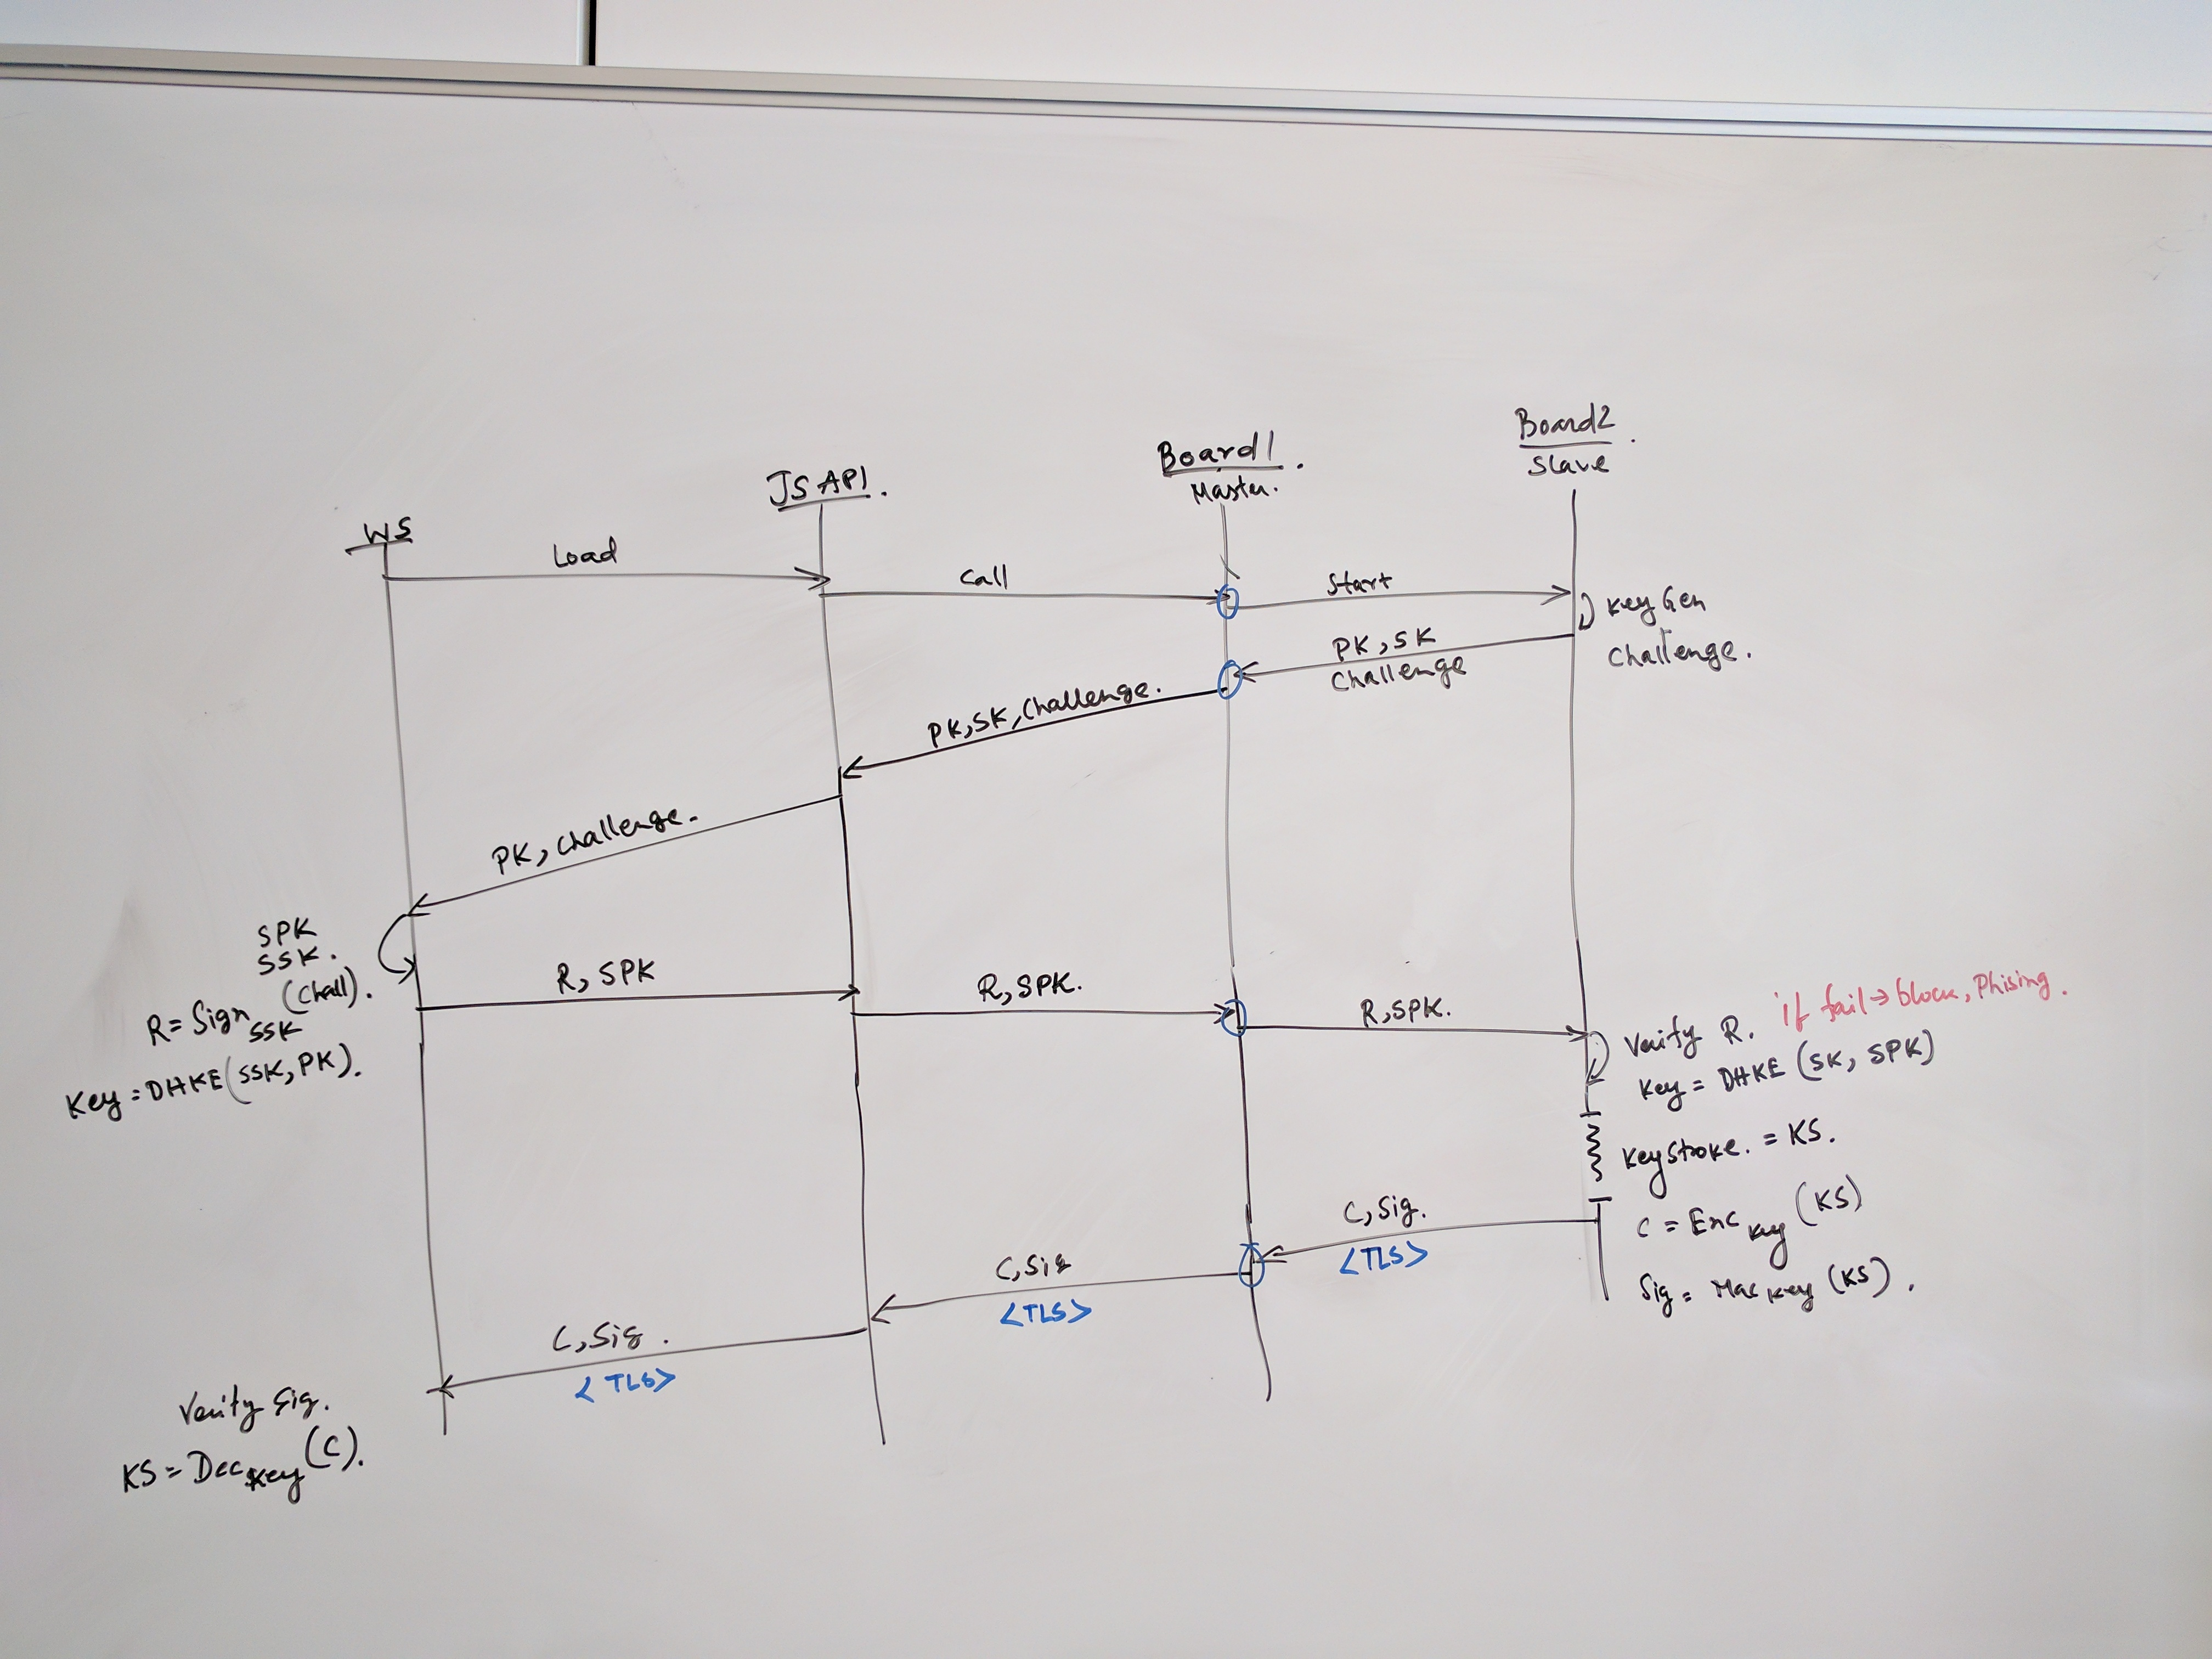
\includegraphics[clip, width=\linewidth]{images/seq.jpg}}
    \caption{Communication sequence between the secure hub and \server}
    \label{fig:seq}maps
\end{figure*}

We propose different solution to solve the problem of phishing and securely
transferring sensitive information to a trusted remote server \server.


\subsection{Secure hub as anti-phishing device}

Here the secure hub acts as a security indicator to detect potential phishing attacks. Our proposed solution is effective both against local and remote phishing attackers. The trust assumption remains similar to other proposed solutions i.e., only the hub and the remote server is trusted. The proposed method works as followed

\begin{enumerate}
  \item User typed a specific address \server\ in the browser. The secure hub record $A_u$ from the browser context. We assume that \server\ supports \webusb\ functionality.
  
  \item When The webpage from the address \server\ is loaded, the secure hub communicates with the web server directly via \webusb\ API.
  
  \item \server and the secure hub the establishes a secure channel (\tls). Over this secure channel the hub requests \server's certificate information along with some challenge (nonce) for freshness.
  
  \item Upon receiving the request, \server sends the certificate along with the nonce and signs the entire message with its private key.
  
  \item If the certificate information and the signed nonce is correct, the secure hub shows a security indicator which identify the web server as the legitimate one. Otherwise it flags the web server as a phishing site.

\end{enumerate}  


\subsection{Dedicated hardware password manager}

This proposed solution eliminate the need of having a security indicator which shows the authenticity of the remote server. In this case the users pre-register her credential in the secure hub. The hub automatically send the credential over a secure channel to the remote server directly if and only if the remote server can prove its authenticity.

 The flow of this mechanism works as below

\begin{enumerate}

  \item Initially the user register with a specific web server and the particular credential in the secure hub and generates a pair (\server, \credential) where \server\ is the remote web server and \credential\ is the corresponding credential. The secure hub stores this pair securely on its memory by encrypting it. We also assume that \server\ supports \webusb\ API to execute this whole process.
  
  \item The secure listen to all user input on the browser (keyboard input and mouse movement). When the user triggers a connection to the specific web server \server\ the javascript snippet of \server\ executes a \webusb\ call to the secure hub.
  
  \item The secure hub establishes a separate \tls connection with the remote server and asks for he public certificate. If \server\ can produce a valid certificate corresponding to its identity, the secure hub shows a security indicator on its display and dispatches the user credential to the remote server. If \server\ fails to produce such certificate, the secure hub flags the communications a phishing attack and blocks further user input.
\end{enumerate}


\subsection{Exchanging sensitive information securely}

This proposed solution is effective against the strongest attacker model where the attacker can compromise host system and the network completely. Apart from the protection against phishing attack, the secure hub additionally transports sensitive information to and from the remote server. It provides confidentiality and integrity. There are several use-cases of this solution and works with any sensitive user input such as credentials, user input in html form etc. The remote server \server which supports \webusb\ specification designs a specific page containing the input fields for the sensitive information in a particular way. It makes all the input fields which handles insensitive data visible in the \html page which can be accessed by the javascript snippets running at the page context. We call these set of insensitive information fields as \insensitive. Rest of the sensitive fields are kept at the server side. We call the set of sensitive fields as \sensitive. As in this scenario we assume the strongest attacker model, we consider the javascript snippet to be completely compromised as the browser can manipulate the snippet.

\begin{enumerate}
  \item Upon rendering the webpage from \server, the browser can only display all the insensitive information fields \insensitive.
  
  \item The \webusb\ API in the javascript snippet communicates with the secure hub and establishes a secure channel (\ssl/\tls) by producing a valid public certificate between the remote server \server\ and the secure hub.
  
  \item Upon establishing a TLS channel with \server, it conveyed all the pensive fields \sensitive\ to the secure hub. The hub displays these fields on the small LCD screen provided with the hub. The use gives input by the connected peripheral (commonly keyboard).
  
  \item Upon receiving and accumulating all the user inputs for all the sensitive fields \sensitive, the hub put itself as the USB pass-through device so that users can provide the insensitive information to \insensitive.
\end{enumerate}

\subsection{Using redirection based method}
  
Here we assume that there exists a trusted webserver (we call it \redir) which helps the secure hub to synchronize with the remote server \server. Apart from synchronization \redir\ also works as a certificate chain for \webusb/\webbt and helps the hub to update its firmware. We also assume \redir\ also serves javascript which includes \webusb\ functionality. The proposed method works as followed:
 

\begin{enumerate}
  \item The user press a button/enter a website address (\server) on the secure hub to initialize the process. Upon initialization, the hub issues a series of keyboard commands to the operating system. The keyboard command includes to open Google Chrome browser to \redir (\texttt{\$google-chrome-stable }\redir).
  
  \item \redir\ serves javascript which directly communicates with the secure hub. The secure hub then directly communicates with \redir\ server provided \redir\ proves its identity by providing certificate. Then the hub and \redir\ establish a \tls channel.
  
  \item \redir\ checks the firmware version and stored public certificates in the secure hub and updates them if required. By this way the hub receives list of revoked and renewed certificates.
  
  \item The hub sends user issued website address (\server) to \redir. Upon receiving this, \redir\ redirects to \server\ location. Now the secure hub expects ro receive communication from \server.
\end{enumerate}

\subsection{Actively detect input field on the webpage}

We assume a malicious host system in our strongest attacker model. In such setting, the attacker can execute local phishing attack, i.e. swapping input fields on the webpage, change the annotation of the field/label on the webpage, modify or drop the input field response etc. The proposed solution works as followed

\begin{enumerate}
  \item As described in tn the other solutions, the server \server\ and the secure hub establishes a secure channel (\tls) leveraging the \webusb\ API.
 
  \item The javascript snippet served by \server contains \texttt{\onSelect} trigger in all of its input fields. The  \onSelect triggers a \http\ web-call to the \server\ relaying the message that which input field is selected by the user.
  
  \item Upon receiving the message from the javascript snippet, \server relay this information back to the secure hub via the dedicated \tls\ channel.
  
  \item The hub records the specific input field identifier ($\mathcal{I}$) sent by the server and then displays it to the secure display module attached to the hub. This display acts as a secure indicator for the user to verify if the malicious host system manipulate any user interaction with the webpage. The hub then records the input keystroke ($ks$) from the keyboard. Encrypt $ks$ and produce ciphertext $\mathcal{C}$ ($\mathcal{C} \leftarrow Enc_{k}(ks)$ where $s$ is the session key of the \tls\ connection).
  
  \item The hub composes a tuple $(\mathcal{I}, \mathcal{C})$, encrypts it and send it to \server.
  
  \item Upon receiving the encrypted tuple, \server\ decrypts it and then process the corresponding information.
\end{enumerate}
 

  
\subsection{Exchanging sensitive information via bluetooth with a smartphone}
\ad{Needs some discussion on this}


